\section{Experimental Results}
\begin{figure*}[htb]
\centering
\subfigure[a] {\label{fig:ite}   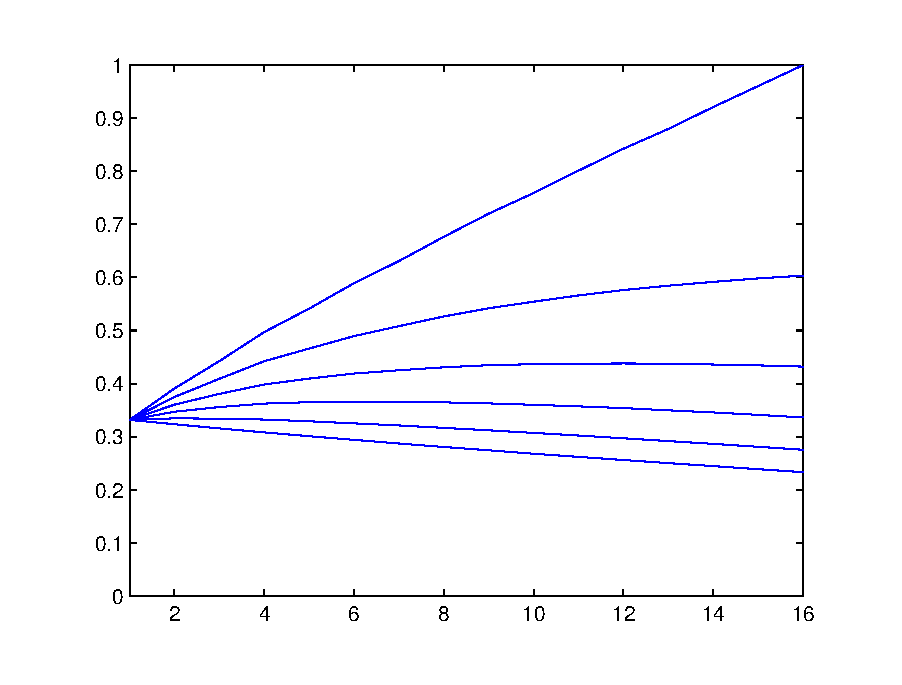
\includegraphics[width=0.32\textwidth]{fig/ppw_16_ite.eps}}%
\subfigure[b] {\label{fig:taylor}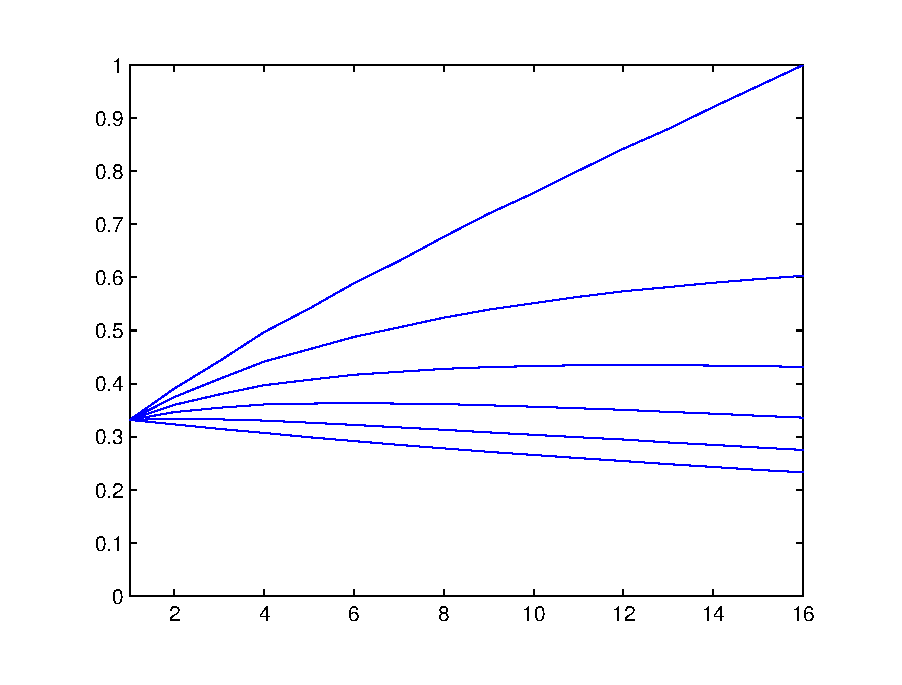
\includegraphics[width=0.32\textwidth]{fig/ppw_16_taylor.eps}}%
\subfigure[c] {\label{fig:tayboo}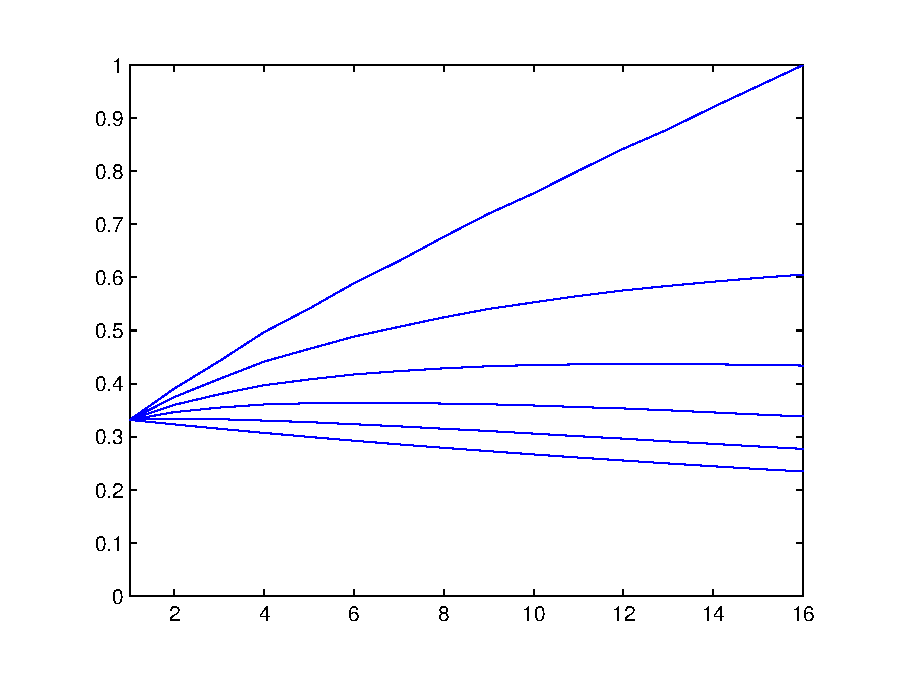
\includegraphics[width=0.32\textwidth]{fig/ppw_16_tayboo.eps}}
\caption{PPW}  
\label{fig:ppw}
\end{figure*}
In this section, we evaluate both accuracy and efficiency of the proposed performance-per-watt estimation technique.

\subsection{Experiment setup}
Through HSPICE simulation, the impact of temperature on device leakage can be characterized. With the collected data, we can obtain the parameters of model through curve fitting as shown in Fig.x. The ambient temperature is set to be \SI{20}{\degreeCelsius}.

For accuracy and speed comparison, we first perform the iteration based power estimation, which is accurate but very time-consuming, therefore we consider it as the golden accuracy baseline (golden for short). Then, two acceleration methods, the taylor expansion based method 